\documentclass[a4paper, twoside, 11pt]{book}

\usepackage{graphicx} % For including figures

% For debugging layout problems
\usepackage{layout}
\usepackage{showframe} % Load the showframe package


% For allowing long url to be broken 
\usepackage{xurl}

% For allowing underline to break across lines
\usepackage{soul}


\graphicspath{{../graphics/logos/}}

% No indentation for new paragraphs because it is a pain to remove it for images
% \setlength{\parindent}{0pt}
\usepackage[skip=10pt plus1pt]{parskip}

\usepackage{setspace}
\onehalfspacing

\setcounter{secnumdepth}{3}

%------------------------
%   Template materials from https://github.com/gramaziokohler/latex_templates/blob/master/research_plan/main.tex


%------------------------
%   Font selection
%------------------------
\usepackage{helvet}

% Select the Helvetica font
\renewcommand{\familydefault}{\sfdefault}

% Hyperlink package
\usepackage{hyperref} % This shows a box around the clickable links, good for debugging.
% \usepackage[hidelinks]{hyperref} % This hides the ugly hyperlink box in the resulting PDF

% -------------------------
% Custom macro to create a (See ... ) section label 
\newcommand{\seeref}[1]{(See \ref{#1} \nameref{#1})}

\usepackage[at]{easylist}


%------------------------
%  Header & Footer 
%------------------------
% \usepackage{color}
\usepackage[]{fancyhdr}

\setlength{\headheight}{14pt}
\setlength{\headsep}{30pt}
\addtolength{\textheight}{25pt}
\addtolength{\topmargin}{-16pt}

% define the plain style for the first page of each chapter
\fancypagestyle{plain}{
	\fancyhf{}% clears all header and footer fields
	\fancyhead[LE,RO]{\thepage}%
	\renewcommand{\headrulewidth}{0pt}%
	% \renewcommand{\footrulewidth}{0.4pt}
	}

\usepackage{titlesec}

% Redefine the chapter style
\titleformat{\chapter}[display]
  {\normalfont\huge\bfseries}{\chaptertitlename\ \thechapter}{20pt}{\Huge}

% define different stypes for title/abstract pages & normal pages
% \fancypagestyle{fancyTitlePage}{
%     \fancyhf{}
%     \renewcommand{\headrulewidth}{0pt}
%     \setlength{\headheight}{70pt}
%     % \setlength\footskip{60pt}
%     \fancyhead[L]{\includegraphics[scale=0.7]{{eth-ita.png}}}
%     \fancyfoot[L]{\raisebox{1cm}[0pt][0pt]{\includegraphics[scale=0.6]{{gkr-bottom.png}}}}
    
% }

% \fancypagestyle{fancyNormalPage}{
%     \fancyhf{}
%     \renewcommand{\headrulewidth}{0pt}
%     \setlength{\headheight}{30pt}
%     \fancyhead[L]{{\includegraphics[scale=0.7]{{gkr-top.png}}}}
%     \fancyfoot[R]{\thepage~/ \pageref{LastPage}}
% }

%------------------------
%  Title & Abstract Page Macro
%------------------------

% signature macro

% \newcommand{\namesigdatehrule}[1]{\par\tikz \draw [gray] (0,0) -- (#1,0);\par}
% \newcommand{\namesigdate}[2][7cm]{%
% \begin{minipage}{#1}%
%     \vspace{1.0cm}\namesigdatehrule{#1}\smallskip
%     \small \noindent\textit{#2}
%     \vspace{0.8cm}\namesigdatehrule{#1}\smallskip
%     \small \textit{Date}
% \end{minipage}
% }
% keywords list macro
% \providecommand{\keywords}[1]{\vspace{1.0cm} \noindent \textbf{\textit{Keywords:\\}} #1}

%------------------------
%   Bibliography Type
%------------------------

% \usepackage[style=authoryear,sorting=ynt,doi=false,isbn=false,url=false,eprint=false]{biblatex}
\usepackage[style=authoryear,sorting=ynt,isbn=false,eprint=false]{biblatex}
			
\addbibresource{Thesis.bib}

%------------------------
%   Author & Advisor Info
%------------------------
% \newcommand{\advisor}{Prof. Fabio Gramazio / Matthias Kohler}
% \newcommand{\researchAuthor}{Your Name}


\title{My LaTeX Test Document}
\author{Pok Yin Leung}
\date{01 September 2023}

\begin{document}
% \layout % For debugging
\maketitle


% \chapter*{Abstract}

This thesis investigates the potential of distributed robotics systems in automating the assembly of timber structures, addressing the challenges of large-scale spatial manipulation and tight-fitting timber joint assembly, which are highly relevant for timber construction.

Leveraging the highly automated process of machining timber parts using automatic joinery machines, the thesis investigates the next knowledge gap in the design-to-production workflow - automatic spatial assembly. Using timber frame structures with integral timber joints as a starting point, this thesis proposed a new fabrication system using distributed robotic tools (DiRT) in collaboration with industrial robotic arms. The crucial breakthrough is the modular and remote operation nature of the tools, allowing the system to assemble a wide variety of timber joints and complex structures.

This thesis also investigated an integrated design workflow. Design validation is identified as a critical aspect of the automated assembly process. This research proposes a practical three-tier validation process to evaluate a design, with quick feasibility feedback provided to the designer during the design process. It takes into consideration geometrical conflicts, robot limitations and tool setup to provide visual feedback on various problems to the designer. 

The research provides a proof-of-concept through the development of three full-scale timber frame demonstrators, each assembled using a single robotic arm and a set of custom-designed distributed assembly tools. The assembly tools include robotic clamps and screwdrivers for different types of lap joints, including planar and non-planar varieties. The findings showcased a viable method to assemble timber structures, mitigating well-known problems such as accumulated assembly error and instability during construction. The results also identified key challenges that are limiting the system efficiency, accuracy, reliability and success rate for the automated process, as well as discovering new opportunities for future research. These opportunities include establishing a generalizable DiRT assembly system, and expanding the range of joint types and building components that can be assembled.

The thesis contributes software tools and system design patterns that are generalizable and reusable within the broader digital fabrication and construction automation community. For example, software for remote robot operation and synchronisation; Data structures and algorithms for robotically assembled structures; Methods for automating parsing designs into robotic programmes; and Task and motion planning techniques for assembly problems.

Ultimately, this research contributes to ongoing efforts to harness the potential of robotics for creating more efficient and sustainable timber construction processes. Paving the way for the widespread adoption of automated construction processes within the architectural industry.


\chapter{Introduction}
\label{chapter:introduction}

The advancement of technology has opened new avenues for innovation in construction.
The use of robots in the assembly of timber structures presents a new frontier in this field.
This interdisciplinary PhD thesis focuses on the integration of industrial robots and Distributed Robotic Tools (DiRT) for the automatic assembly of timber structures.
Specifically, timber frame structures with integral timber joints. 

Despite the potential benefits that automation could bring to the construction industry, the necessary technology to achieve this goal remains unknown. The objective of this thesis is to embark on a journey of discovery and innovation that will contribute to the advancement of knowledge in the field.
By combining interdisciplinary approaches from timber construction, computational design and robotics, this research will provide insights into the technical and operational aspects of the automatic assembly process, as well as its potential benefits and challenges.
Through the development of novel solutions and empirical construction experiments, this PhD thesis aspires to shape the future of construction and contribute to the interdisciplinary field of digital fabrication, between architecture, construction and robotics.

\section{Timber Frame Construction}
\label{section:introduction-timber-frame-construction}

Timber construction has been used historically in many cultures with an ample supply of trees.
Timber is a remarkable construction material because of its very high strength-to-weight ratio.
It can withstand tension and compression, making it suitable for different structural roles. Moreover, timber can naturally reach lengths of many metres, which provides tall columns and long beams for the construction of architectural structures at various scales.
Historically, many types of construction methods have been developed. The focus of this thesis is timber frame construction which refers to a range of timber construction methods used as early as the 12th century until the early 20th century \parencite{sobonTimberFrameConstruction1984}.

\subsection{Defining Characteristics}
\label{subsection:introduction-defining-characteristics}

Timber frame construction can be understood as a set of techniques that have evolved over time. Carpenters have experimented with different joint designs, structural arrangements and methods to frame walls, floors and roofs. While these techniques evolved independently in different civilisations, similar material behaviour (e.g. anisotropicity of wood, prone to decay) and similar design goals (e.g. weather protection) resulted in many similarities between them \parencite{zwergerWoodWoodJoints2012}.
While there are still differences between regional practices (caused by regional timber species, weather, local culture and ornamental preferences), the type of timber construction that dominated the pre-industrial era (especially in Europe, North America, and Japan) share similar defining characteristics, such as \textit{large timber sizes}, \textit{integral timber joints}, and \textit{post-and-beam framing}. 
These characteristics make timber frame construction ideal for studying automatic assembly.
As such, this thesis is not referring to the timber frame construction of a specific location or time period, but rather to the general use of these three defining characteristics of timber frame construction.

\subsubsection{Large Timber Size}
\label{subsubsection:introduction-large-timber-size}

The first defining characteristic of timber frame construction is large timber sizes.
Historically, this is the result of using a whole harvested tree trunk as a structural member instead of laboriously cutting them into smaller pieces.
It was only after the industrialisation of sawmills that timber could be efficiently cut into smaller dimensions.
Around the same time, the depletion of large trees in Europe and America prompted the more contemporary invention of stick framing construction (i.e. balloon framing and platform framing) that uses dimensional lumber (e.g. 2x4 inch “two-by-four” studs). Later as timber glue technology improved, the use of glue-laminated timber (glulam), Laminated Veneer Lumber (LVL) and other engineered timber products began to appear and allowed the manufacturing and use of large timber elements again.
In this thesis, the assembly of both solid timber and engineered timber is investigated.
The nominal size being used is 100mm x 100mm square profile \seeref{subsection:exploration-1-scope-for-initial-exploration-round}

\subsubsection{Integral Timber Joints}
\label{subsubsection:introduction-integral-timber-joints}

The second defining characteristic in timber frame construction is the use of integral timber joints (ITJ), where the jointing geometry is carved into the material. Structural load is transmitted from element to element directly through contact pressure over the mating surfaces of the joint. The design of these joints has been refined empirically throughout history, converging into specialised designs according to which structural elements they are connecting \autocite{jacksobonHistoricAmericanTimber2014}. It is common for a joint to serve multiple purposes and thus withstands different types of loads, such as self-weight and live forces. Different ‘geometrical features’ can therefore be incorporated into the connection to meet different force conditions. For example, a lap joint for a floor joist can be combined with a dovetail feature to provide tension resistance.
These joints are typically dry-fitted\footnote{Historical glue technology could not withstand structural forces} and held in place due to interlocking geometry and gravity.
Additionally, it is possible to include metal components in integral timber joints.
This is more common in contemporary design, where metal screws, dowels and tie rods are used to improve joint capacity or to reduce the need to cut complicated joinery.
For the purpose of studying automatic assembly, integral timber joints provide a unique advantage because they can be prefabricated with high accuracy \seeref{subsubsection:introduction-automatic-machining-of-timber-joints} and are quick to install.
In this thesis, the assembly of dry-fitted joints both with and without fasteners is explored.

As of today, there is no single consensus in the nomenclature of timber joints as different cultures have historically named their joints using different methods \parencite{satoCompleteJapaneseJoinery1995,seikeArtJapaneseJoinery1977a,sumiyoshiWoodJointsClassical1991}. The first naming convention (commonly used in American and European traditions) is based on the location of the joint and the structural elements it connects to, for example, ‘floor joist joint’ or ‘tying joint below plate’. The second naming convention is based on the joint's geometrical features, for example, ‘dovetail joint’ or ‘scarf lap joint’. Some unique joint designs could also be named according to the use in a famous building. For example, Osaka-jo-otemon-hikae-bashira-tsugite refers to Osaka Castle-Otemon Gate's pillar splice. For the purpose of studying assembly problems, this thesis proposes the use of a different convention that is based on the assembly direction related to the joint \seeref{subsection:exploration-1-lap-joint-classification-by-assembly-direction}.

Figure \ref{fig:example-timber-frame-on-ground} shows timber frame components being assembled on the ground. Notice the use of large timber sizes and integral timber joints. 

\begin{figure}
    \centering
    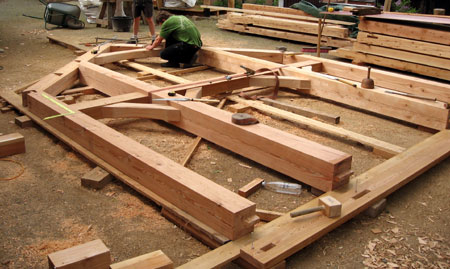
\includegraphics[width=0.99\textwidth]{images/01/Fachwerk_Abbund.jpg}
    \caption[Example of timber frame components being assembled on the ground]
    {Example of timber frame components being assembled on the ground \\
        \footnotesize{(Credits: CC AS 4.0 Licence photo by Georg Hefter - Traditionelles Fachwerk und Timberframe im Vergleich auf georghefter.de)}}
    \label{fig:example-timber-frame-on-ground}
\end{figure}

\subsubsection{Post and Beam Structure}
\label{subsubsection:introduction-post-and-beam-structure}

The third defining characteristic of timber frame construction is post-and-beam structural framing \parencite{jacksobonHistoricAmericanTimber2014,sobonTimberFrameConstruction1984}. The use of large timber sizes in timber frame structures allows them to be strong enough without the use of continuous load-bearing walls. The main benefit is the flexible arrangement of floors and walls to suit different architectural programmes. 
On the other hand, integral timber joints are generally weak in rotational stiffness, causing the joints to behave kinematically. Therefore, diagonal bracing is often introduced to fully or partially triangulate the structure to improve structural stiffness. Being limited by the joint design, these bracings function primarily in compression. It is, therefore, common to design the bracings in complementary pairs to resist dynamic wind loads coming from opposing directions. While some architectural designs may find the intrusion of diagonal bracings obtrusive to usable space, these diagonal bracings are highlighted on the facade as ornamentation in half timber designs \parencite{gernerFachwerkEntwicklungGefuege1979}. In this thesis, the demonstration structures are designed with similar structural principles, specifically the use of structural triangulation in the design offered unique stability advantages during the robotic construction process \seeref{subsection:exploration-4-deformation-awareness-and-error-correction-by-triangulation} \seeref{subsubsection:exploration-4-global-correction-approach}.

Figure \ref{fig:half-timber-frame-example} shows an example of a half-timber style timber frame house in Soest, Germany. Notice the exposed diagonal elements on the facade.

\begin{figure}
    \centering
    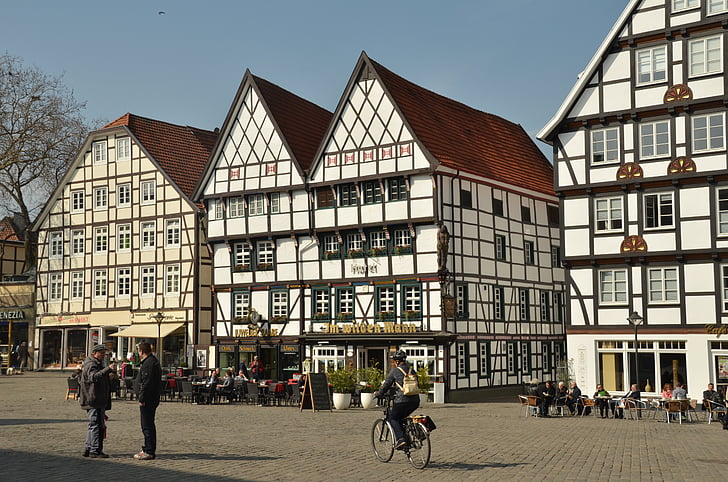
\includegraphics[width=0.99\textwidth]{images/01/germany-soest-architecture-timber-framed-preview.jpg}
    \caption[Example of a half-timber style timber frame house]
    {Example of a half-timber style timber frame house \\
        \footnotesize{(Credits: Licence-free photo, retrieved from \url{https://www.hippopx.com/en/germany-soest-architecture-timber-framed-half-timbered-house-square-city-402214} , n.d.)}}
    \label{fig:half-timber-frame-example}
\end{figure}


    
\subsection{Current Practice of Timber Frame Construction}
\label{subsection:introduction-current-practice-of-timber-frame-construction}

Timber frame construction was once the dominant building method, but it gradually declined in popularity during the 19\textsuperscript{th} and 20\textsuperscript{th} centuries. The advent of industrialization and mass production led to the availability of cheaper building materials such as steel and concrete, which were faster and easier to use. Even within the timber construction sector, newer construction methods that use dimensioned lumber, glulam, LVL, and Cross Laminated Timber (CLT) have replaced timber frame construction. However, in recent years, as more people are aware of the environmental benefits of wood construction, interest in timber frame construction is increasing again as an alternative way to construct with timber. 

Advancements in engineering and design, as well as increased availability of sustainably sourced timber, have helped to make timber frame construction a more viable option for modern building projects. Timber frame components can be prefabricated off-site, which can reduce construction time and costs while also minimising waste and environmental impact. The use of dry-fitted integral timber joints reduces the number of fasteners and components involved, meaning less metal consumption and quicker installation on-site. Furthermore, timber frame structures can be aesthetically pleasing as they often expose the beautiful timber material and reveal the structural load paths. When the joint details are exposed, they can evoke a feeling of tradition and craftsmanship and are often well-appreciated by those who inhabit the building.

\subsubsection{Automatic Machining of Timber Joints}
\label{subsubsection:introduction-automatic-machining-of-timber-joints}

Between the years of decline and its recent resurgence, a number of technological improvements have made timber frame construction more efficient and competitive. One of the major advancements has been the use of automatic joinery machines for carving integral timber joints. Traditionally crafted with hand tools, these joints were labour-intensive and required highly skilled craftsmen that could work precisely.\footnote{The task of marking and setting out was considered the most critical and is often performed by the master carpenter. Other carpenters would prepare materials and carve joints using hand tools such as saws, planes, chisels, and drills.}
Since the invention of automatic joinery machines, the production of timber joints has become highly automatic \parencite{hanshundeggeragCorporateDevelopment2023}. These machines often feature interchangeable cutting tools and can create many types of joints at the beam ends and along its length. Today, the machining of timber joints is very mature and efficient. The automatic joinery machines are controlled by Computer Numeric Control (CNC) technology and can follow a digital program to create timber joints of different designs at different positions. The program can be quickly changed to create different timber elements used for an entire building. \seeref{subsection:introduction-programming-digital-fabrication-machines}

This thesis capitalises on the accuracy and prefabrication efficiency provided by the automatic joinery machines. Accurate parts are highly advantageous for robotic automatic assembly because they ensure accurate manipulation and precise integration. By using prefabricated timber parts with accurately machined integral timber joints, this thesis aims to create a highly automated assembly process, reducing the manual labour needed for adjustment and adaptation. 

\subsubsection{Assembly by Carpenters}
\label{subsubsection:introduction-assembly-by-carpenters}

Although the production of timber frame components is automated, the assembly of the structure is still predominantly manual \parencite{willmannNewParadigmsAutomatic2016}. It usually takes a team of carpenters to assemble a timber structure.

Timber frame structures are almost always assembled on-site due to the nature of their post-and-beam structural system, which favours long and unbroken elements. This means that pre-assembling multiple elements off-site, is not practical because it will result in assemblies that are too big for transportation. 

Below is a summary of the tasks that carpenters perform during the assembly of a timber frame structure, focusing on the structural elements:

\begin{itemize}
	\item \textbf{Sorting timber parts --} Prefabricated timber parts are typically delivered on-site in bundles that correspond to different assembly stages. Many of the components are geometrically unique because of the layout of the joints. Carpenters must identify the correct location for each element based on label and markings on the parts and sort them according to the assembly sequence.

	\item \textbf{Manipulating timber parts spatially --} Post, beam and diagonal bracings are assembled in different spatial (3D) orientations. Carpenters must identify and orient the parts correctly when bringing them to their assembly location.

	\item \textbf{Applying forces --} Because of contact friction and deformation, carpenters may need to apply force to the joints using hand tools. They may use common generic tools such as mallets and screwdrivers (pulling with a screw), or specialise tools such as ratcheting joint pullers. 

	\item \textbf{Aligning mating joints --} Multiple carpenters are often required at every mating joint. They may have to push or pull the already-assembled elements for alignment. 

	\item \textbf{Synchronous Assembly --} During the closure of the joints, the carpenters also ensure parallel and synchronous motion to avoid jamming.

	\item \textbf{Adjusting timber joints --} If a timber part does not fit. Carpenters can remove material or shim gaps. These types of problems are rare with CNC fabricated parts, but can sometimes occur due to poor machining tolerance, design error, machine-programming error, and shrinkage or expansion after machining.

	\item \textbf{Placing fasteners --} Some contemporary joint designs include screws, nails, or dowels.

\end{itemize}

These tasks are the focus of the automated assembly process pursued in this thesis. The challenges of each task are analysed and presented in the next chapter \seeref{section:challenges-mechanical-challenges}.

\subsection{New Opportunities for Timber Frame Construction}
\label{subsection:introduction-new-opportunities-for-timber-frame-construction}

Compared to other newly developed construction methods with a higher degree of prefabrication, the on-site timber frame construction is less economically competitive. For example, modular floor and wall construction allow more components to be assembled off-site (e.g. insulation, windows, doors), which reduces the time and cost associated with on-site work. Volumetric prefabrication (e.g. modular timber construction), which pre-assembled an entire room, further allows the installation of wiring, plumbing, and interior finishes in a factory \parencite{adelDesignRoboticallyFabricated2018}. 

Despite the lack of prefabrication advantages, timber frame construction enjoys greater design freedom because there are fewer transportation constraints when moving linear timber elements than moving a preassembled room-sized timber module. This freedom is essential in creating large-span structures or shell structures where sub-assemblies cannot be effectively transported. In addition, latest timber frame designs have already been able to integrate contemporary building requirements such as plumbing, electrical wiring and insulation that meets building codes \parencite{bensonTimberframeHomeDesign1988}. Therefore, the exploration of automatic assembly for timber frame structures could potentially keep these benefits without the associated penalty of on-site manual work.

\section{Architectural Design to Production}
\label{section:introduction-architectural-design-to-production}

In recent years, the fields of architecture and construction have seen a growing interest in automating various stages of the design and production process. This trend is being driven by the potential benefits of automation, which include increased efficiency, higher precision, and improved quality control. Automation can also help to reduce labour costs, minimise waste, and improve safety on construction sites. While automation has already become common in the manufacturing industry, its adoption in architecture and construction has been slower due to the unique challenges and complexities in the construction sector. Most commercialised examples are limited to prefabrication of small or planar architectural components while only a handful of research projects have attempted to use robotics for structural scale spatial assembly. Therefore, this thesis aims to expand knowledge in this area, starting with the assembly of timber frame structures.

This section will present a brief history of how the timber construction industry transitioned towards digital design and automated production, leading to the current state of the art practices. It is an important starting point to understand whether the assembly process will also undergo such a transition. 

\subsection{Automation from Manufacturing to Construction}
\label{subsection:introduction-automation-from-manufacturing-to-construction}

The beginning of automation started with the manufacturing industry. It involves the use of machinery or computer systems to perform tasks that would otherwise be done by human labour. Without going into details, it typically involves the use of sensors, actuators and control systems to reduce or eliminate the need for human intervention \parencite{nofSpringerHandbookAutomation2009}. It has become a widely adopted practice in the manufacturing industry due to its benefits such as increased efficiency, improved quality, and reduced costs. With automation, the production process can run continuously with a predictable production schedule.

The successful implementation of automation is closely tied to the design and operation of production machines. Since the beginning of industrial automation, automatic machines have undergone several evolutions that are characterised by their features, modes of operations and benefits. Early automatic machines were mechanical systems that performed repetitive fixed operations. Their motions were often defined mechanically through the use of components such as linkages, cams and conveyor belts. Because of this, their motions cannot be easily modified without changing parts. These machines favour high-volume, low variability products that represent the mass-production paradigm of Industry 2.0\footnote{The First Industrial Revolution, aka. Industry 1.0, began in the late 18th century where mass production was carried out by machines powered by water and steam.}.
While some of the earlier machines still require an operator, later machines would contain control systems that are capable of performing cyclic actions on their own. After the introduction of electricity, the use of logic controllers became more common and allowed the machines to make decisions using sensors and signals. The increased level of autonomy allowed further reduction of operator interventions. This type of automation is a typical defining characteristic of Industry 3.0 \parencite{mengesNewCyberPhysicalMaking2015,yinEvolutionProductionSystems2018}. 

Invented in the 1950s and popularised in the 1960s, Computer Numeric Control (CNC) technology further increased the flexibility of machines, such as the aforementioned automatic joinery machines and industrial robotic arms. The motion of CNC machines are defined through the use of a digital ‘program’ such that their motion can be easily modified when products are changed \parencite{wardAutomaticProgrammingNumerically1959}. This is often achieved by incorporating a computerised digital control. The ability to change design quickly eventually led to the mass-customisation paradigm of Industry 4.0. In extreme cases, products can even be unique from piece to piece, resulting in the ‘batch size of one’ paradigm \parencite{wardAutomaticProgrammingNumerically1959}.

The adoption of automatic machines has changed the nature of work from labourers to operators and increasingly towards engineers and programmers \parencite{nobleForcesProductionSocial1986}. While this shift may be difficult for workers unable to acquire a new skill set, it improves the general labour working conditions in the longer term \parencite{stromquistWorldDevelopmentReport2019}. For example, by reducing repetitive manual tasks or avoiding working in dangerous environments. 

\paragraph{A Factory for Making Buildings}

\label{subsubsection:introduction-a-factory-for-making-buildings}

At a larger scale, the concept of automation can be applied to connect different machines together to autonomously regulate production flow. There are two types of connections involved, the first is physical connections, such as using conveyor belts and robotic arms to move parts between machines. The second is logical connections, such as programmable logic controllers forming complex logic networks. In extreme cases, the term \textit{lights-out factory} or \textit{automatic factory} was used to describe large production facilities that are able to sustain continuous production with very few or infrequent operator involvements \parencite{nobleForcesProductionSocial1986,walkerAutomaticFactoryCase1957}. 

Recently, the introduction of large-scale concrete 3D printing technology has brought the automatic factory vision within reach for the architecture and construction community \parencite{ngoAdditiveManufacturing3D2018}. While large-scale 3D printing processes are still at the research stage, smaller 3D printers have already achieved full autonomy, allowing users to press a start button and come back later for the completed parts. The idea of a black-box fabrication machine where design information and raw materials are the only input, was hypothesised to be the future mode of production that can make almost anything \parencite{gershenfeldHowMakeAlmost2012, gershenfeldInternetThings2004}.  

Started in the late 1970s, Japan’s large construction contractors have begun developing robots capable of performing construction tasks. The initial robots were single-task construction robots, designed to perform one specific function, such as finishing concrete, welding, or spray painting \parencite{potterJapanSkyscraperFactories2022}. Starting in the mid-1980s, Japan’s construction robot development shifted away from individual robots, and towards creating an entire robotic construction site \parencite{maedaCurrentResearchDevelopment2005}. The process often makes use of a high number of prefabricated components and focuses on improving the speed for the assembly task. Studies have found that the productivity gain is often apparent when constructing a tall and repetitive building \parencite{linnerAutomatedRoboticConstruction2013,potterJapanSkyscraperFactories2022}. 

While the automated systems seen in Japan are mostly designed for steel and reinforced concrete structures, this thesis studies what it would take for timber construction to achieve a similar level of automation. 

\subsection{Automatic Assembly in Timber Construction}
\label{subsection:introduction-automatic-assembly-in-timber-construction}

In recent years, interest in exploring automatic assembly for timber construction has grown. This was driven by the potential for increased efficiency, precision, and sustainability. Despite the advancements in fabrication techniques, particularly with the advent of CNC technology, the assembly process still presents challenges that industry professionals and researchers are working to address \parencite{willmannNewParadigmsAutomatic2016}.

In the industry, the advancement was mainly focused on the assembly of flat-stackable prefabricated parts, such as light-framed timber floors and walls. Companies like Biesse, Homag, and Weinmann have been developing advanced machinery and automated solutions for timber processing and assembly \parencite{kooTechnologyGapsAchieve2021}. These systems are often large-scale installations similar to a manufacturing production line and are custom engineered for a specific factory. The entire system can include separate material processing stations, such as cutting and joinery machines and for linear timber and panel saws for sheet materials. Processed materials would merge into a central assembly line and be assembled using nails, screws and adhesive depending on its design. Additionally, companies like MiTek and Randek have been focusing on the prefabricated housing sector, developing automated systems for the assembly of timber roof trusses \parencite{ianharveyRoboticArmsAI2018}. 

Despite these groundbreaking efforts, the challenges for spatial timber assembly is rather unique \seerefii{section:challenges-mechanical-challenges}{section:challenges-computational-and-design-challenges}. These challenges are complex, interdiscipline and are often specific to the construction system. This makes it hard to generalise solutions between different type of constructions. For example, despite having high demand in the industry, the spatial assembly of planar walls to create volumetric timber modules is still performed manually; timber frame structures, despite existing for a long time, still have no automatic assembly solutions. As the demand for sustainable building solutions continues to grow, and the skilled labour market continues to shrink, the exploration of automatic assembly methods for timber construction is urgently needed. 

Several innovative research projects have emerged in recent years, addressing the challenges of spatial manipulation of linear timber elements. For instance, the pioneering work conducted by Gramazio Kohler Research at ETH Zurich has shown the potential of using industrial robots to assemble complex timber structures. While early explorations were limited to a 2.5D stacked assembly approach \parencite{apolinarskaSequentialRoof2016, gramaziokohlerresearchethzurichStackedPavilion2009, helmInSituFabricationMobile2014}, many later projects addressed 3D spatial manipulation. For example, the first two-story robotically assembled structure \parencite{eversmannRoboticPrefabricationTimber2017}, the volumetric timber modules of the DFAB House \parencite{adelDesignRoboticallyFabricated2018, thomaRoboticFabricationBespoke2018}, and many other spatially assembled timber structures \parencite{apolinarskaRoboticAssemblyTimber2021, eversmannRoboticPrefabricationTimber2017, helmAdditiveRoboticFabrication2016, helmreichRoboticAssemblyModular2022,willmannNewParadigmsAutomatic2016}. Similarly, other research institutes have demonstrated the capabilities of using industrial robots to assemble prefabricated timber plates spatially \parencite{robellerRoboticIntegralAttachment2017, rogeauRoboticAssemblyIntegrallyAttached2023} and to assemble modular timber cassette systems \parencite{alvarezBUGAWoodPavilion2019, claypoolAutomationDiscreteExploring2021}.

This thesis aims to contribute to the ongoing efforts to advance the state of the art in this domain. Using timber frame construction as a starting point, the assembly problems are studied and addressed in a holistic way, with the intention to improve the understanding of these problems and for generalizable solutions to emerge.

\subsection{From Automation to Digital Fabrication}
\label{subsection:introduction-from-automation-to-digital-fabrication}

In the 1990s, various computer programmes that were intended for animation (e.g. Alias Wavefront, Maya) and engineering (e.g. Catia, later DigitalProject) were adopted by the architectural community for modelling geometrically complex buildings. This partially triggered the bloom of freeform architectural designs that are made famous by architects such as Frank Gehry, Zaha Hadid, Santiago Calatrava. For example, \textit{Fishdance Restaurant, Kobe (1989),  Guggenheim Museum Bilbao (1997), Walt Disney Concert Hall (2003)},and \textit{ Louis Vuitton Fondation (2014)}.\textit{ }

The immediate implication of freeform architectural designs is the need to produce geometrically complex components. This was addressed by the use of CNC machines that can follow arbitrarily complex paths. However, freeform architectural designs also implies the need to produce a large amount of non-repetitive components. At the component level, this is similar to the mass-customisation paradigm in manufacturing. However, in order to create the unique CNC programmes for the production process, Computer-aided design (CAD) and computer-aided manufacturing (CAM) software became an indispensable part of the production workflow \parencite{sheldenDigitalSurfaceRepresentation2002}. 

\textit{CAD software} allows architects and construction engineers to create 2D or 3D models of buildings, including the detailed geometry of each building component. Using these models, production engineers use \textit{CAM software} to generate toolpaths for the CNC machines. Because of the non-repetitive geometry, each component requires a unique programme for the CNC machines for operation and unique drawings for the workers to perform the assembly and inspection. This eventually leads to a workflow where not only are the machines automated, but the production of information is also automated. This new mode of production became what is known now as \textit{Digital Fabrication}.

The basic workflow for CAD is called direct modelling, where designers explicitly create and modify geometry in a linear workflow. This can be analogous to the ‘drawing’ process in architectural design as the designer interacts with the computer program over a graphical user interface (GUI) in an interactive way. The designer can use functions offered by the CAD to add or modify geometry. A more advanced workflow is \textit{parametric modelling}, where the history of modelling operation is saved for later reuse. This can be as simple as a ``Macro", where multiple functions are chained for easy access, or as complex as to define geometry based on a chain of functions and input parameters. This can be analogous to writing a mathematical equation with functions and variables. By changing the input values to the variables, the equation can be used to represent many possible outcomes. Therefore the output of a parametric model is dynamic and can be regenerated if necessary. Designers typically create a parametric model in one of the two ways. The first method is by demonstrating the modelling or computation logic to the CAD programme while the programme ‘records’ the logic which can be reused later. The second method is to create a symbolic description, similar to computer programming. This is often called \textit{Scripting} and is often used for more complex logic. Depending on the CAD programme, this symbolic script can be written in one of the many programming languages (e.g. C$\#$, Python) or, more recently, in a graphical programming interface (e.g. Grasshopper, Dynamo). 

There are two important benefits of a \textit{reusable CAD workflow}. The first is to save time when modelling large amounts of geometrically similar (but not identical) parts. The second benefit is the ease of making design changes. For example, the designer only needs to change the inputs for the CAD programmes to update the downstream documents automatically. These can include 3D models of components, 2D drawings and assembly instructions. In recent years, the popularity of parametric workflow has shaped the way designers interact with the design process. Instead of focusing on the final outcome, the automated workflows allow them to design the geometrical logic first before adjusting the input parameters to achieve the desired geometry \parencite{jabiParametricDesignArchitecture2013}. In addition, measurement and evaluation logic can also be incorporated into the script, allowing designers to be more informed about their designs. Complex relationships between geometry and structure can also be scripted to allow an intuitive and interactive design process \parencite{pottmannArchitecturalGeometry2007, woodburyElementsParametricDesign2010}. This design process that is supported by parametric modelling is often called \textit{Parametric Design}.

\subsection{Programming Digital Fabrication Machines}
\label{subsection:introduction-programming-digital-fabrication-machines}

Reusable workflows have also been extended to the CAM software to generate machining programmes automatically. This refers not only to the automated creation of toolpaths from a part geometry, but also the automatic decision-making to choose machining strategy, tool choice, machining sequence, and machining speeds. In the architectural context, this type of workflow has been used for cutting 1D profile materials and 2D sheet materials for geometrically complex facade systems used in free-form buildings \parencite{eigensatzPanelingArchitecturalFreeform2010, sheldenDigitalSurfaceRepresentation2002}.

In timber construction, the aforementioned automatic joinery machines were invented before the digital fabrication revolution \parencite{hanshundeggeragCorporateDevelopment2023}. Programming work for these machines was initially done by manually entering joint parameters (such as joint type, size and location on the beam). However, this work was soon automated by CAD (e.g. Cadwork 1988) and CAM (e.g. LignoCAM) software that was developed for the timber industry \parencite{schwinnManufacturingPerspectives2016}. Timber-specific CAD software improved efficiency for modelling matching pairs of joints across different elements and reduced the risk of design errors. While the CAM software is responsible for converting the joint features of the 3D model (such as cutouts and drill holes) into machine-specific programmes for the automatic joinery machines.

In the early days, CAD and CAM functionality were integrated into the same programme. However, as more machine manufacturers such as Biesse, SMC Group, and Homag started to make automatic joinery machines, open file formats were developed to allow different CAD, CAM and automatic joinery machines to work interchangeably. The current industry standard is the BTL (2006) and later BTLx (2015) format for data exchange. They were developed by a collaborative effort from the industry to create a specialised format for describing timber components. For example, it can represent timber grain directions, glulam orientation and joint machining tolerance that would otherwise not be possible using generic 3D model formats \parencite{lignocamBTLxWhatIt2020, design2machineHistoryDataTransfer2023}. 

The design-to-production workflow would typically start with a timber engineer that creates 3D models of the arrangement of beams and joints in the CAD software. Design iterations would happen within the CAD programme until architectural and structural requirements are met. Construction planning would also be performed in the CAD environment for specifying the production schedule and assembly sequence. The description of the beams and joints would then be passed to machine-specific CAM software by using, for example, the BTLx file format. The CAM programme would be able to recognise the timber elements and their joint details and make machining decisions specific to the fabrication machine setup. For example, to choose a suitable saw, mill bit or drill bit size from a collection of available tools; or to decide whether a hole is drilled or milled.

A production engineer, who has intimate knowledge of the machine setup, is often involved in defining the rules that the CAM software would follow. The ruleset would include a description of machine limitations, available tools, material choice, desired machining quality and production sequence. Conceptually, this is similar to the reusable CAM workflow mentioned above with a similar intention to automate the CAM software, to handle a large number of geometrically unique elements. 

Hypothetically, the assembly process studied in this thesis can also adopt a similar workflow. There is a strong similarity between creating machining programmes and creating robotic assembly programmes. Both of them are specific to the machine setup (e.g. robot kinematics), machine limitation (e.g. avoiding collisions) and tools setup (e.g. end effectors). It also needs to overcome the complexity of making decisions according to unique geometry. Therefore, this thesis adopts the parametric modelling and reusable workflow from machining as a starting point and apply it to robotic timber assembly \seeref{subsection:exploration-3-workflow-for-generating-assembly-programmes}. 

\subsection{Fabrication-aware Design}
\label{subsection:introduction-fabrication-aware-design}

\begin{quote}
	``While digital models are easily created, the actual fabrication and construction remain a challenge.'' \parencite{pottmannArchitecturalGeometryFabricationAware2013}
\end{quote}

The disconnection between design and fabrication is the source of numerous frustration that forced many geometrically complex projects into a ‘redesign’ phase after the reality of fabrication and construction limitations was imposed. This redesign process is known as rationalisation \parencite{pottmannArchitecturalGeometryFabricationAware2013}. A rationalisation is a design negotiation between keeping the design intent and reducing fabrication costs. It invariably led to a loss of fidelity. A better approach would be to incorporate knowledge of the actual construction process during the design stage; this is known as construction-aware or fabrication-aware design.

In the current architecture and construction industry, the role of evaluating constructability lies in the hand of a construction engineer. Very often it is a single-direction workflow that is difficult to accommodate frequent design changes. As architectural design practices migrate towards a digital workflow, there is a growing interest to automate the evaluation process. One common approach is to encode the knowledge of the fabrication constraints as computational algorithms, which can be computed automatically within the CAD design software. Feedback can therefore be provided as quickly as possible for the designers, which gives them a better chance of pushing designs closer to fabrication limits yet without violating them. 

These automatic checks, also known as design validation, are particularly useful when dealing with designs that have many unique parts (that would otherwise need to be checked individually) or when the fabrication limitations are complex or obscure. They also help avoid human errors and mistakes that are costly to fix downstream. 

While the concept of fabrication-aware is often used to check prefabricated components and machining processes, the concept can hypothetically be applied to a robotic assembly process. For example, robot reachability, payload, and collision. As long as a constraint can be modelled as a computable algorithm, it can be checked automatically. However, in practice, not all checks are easy to model and certain behaviour requires advanced simulation to model. This will be further elaborated in the next chapter \seeref{section:challenges-computational-and-design-challenges}. However, it is exactly because of this complexity that makes it difficult for a designer to evaluate them manually. Therefore in the context of this thesis, one of the main explorations is to study whether robotic assembly processes can be checked automatically and whether a fabrication-aware design workflow is feasible. 

The following sections present two case studies in the field of digital fabrication. They provided a positive indication that an integrated design and fabrication workflow is achievable.

\subsubsection{Case Study - Automatic CNC Machining Programme}
\label{subsubsection:introduction-case-study-automatic-cnc-machining-programme}

The first case study is a comparison between robotic assembly and machining processes. Assembly robots are similar to complex milling machines with multiple axes in the sense that they are both capable of making complex movements. However, they are also prone to programming errors that can cause expensive damage. Therefore, when creating toolpaths, a CNC programmer will often rely on the multitude of checking algorithms offered by the CAM software to catch potential problems. It is common for a CNC programmer to resolve production problems separately, within the scope of modifying machine parameters, tooling or cutting strategy. It is only until the attempts are exhausted that the programmer will suggest design changes to the designer. 

The culprit of this long evaluation cycle is that the current practice of creating toolpaths requires a lot of manual input. On the one hand, this offers many optimization possibilities for the machining process but at the same time makes feasibility evaluation very complex. In order to address this problem, researchers have identified the need to combine the automatic generation of toolpaths and automatic validation \parencite{garciaProcessPlanningBased2011,sheenMachiningFeatureRecognition2006, joshiGraphbasedHeuristicsRecognition1988}. These methods have already been adopted by companies offering machining services to generate CNC programmes automatically. This enabled them to provide almost-instant price quotations for parts solely based on a geometrical model. 

Similar to the hypothesis proposed before \seeref{subsection:introduction-programming-digital-fabrication-machines}, there are a lot of similarities between an assembly process and a machining process. Perhaps the same automatic generation and validation principle can be applied to robotic assembly processes to enable a more integrated workflow.


\subsubsection{Case Study - Automatic Slicing for 3D Printing}
\label{subsubsection:introduction-case-study-automatic-slicing-for-3d-printing}

Another parallel can be drawn between robotic assembly and additive manufacturing. Fused Deposition Modeling (FDM) Printers are mechanically simple devices that can create 3D parts by stacking 2D slices. However, the generation of toolpaths (a.k.a slicing) requires advanced algorithms to determine optimal toolpath, layer height, infill density, print speed, and other settings based on the geometry of the model, the type of printer, and the material being used. Additionally, the slicer software needs to take into account various non-linear factors that can affect the quality of the printed object, such as the cooling rate of the material, the shrinkage of the material as it cools, and the adhesion of the material to the print bed. Slicers may also include features such as support generation, which creates structures to support overhanging features of the model during printing. 

As a result, slicers can be quite complex and require a significant amount of tuning and customization. Nevertheless, pre-tuned slicers for commercially available printers can produce satisfactory results for almost any 3D geometry. In many cases, they are fully automatic upon the reception of a CAD model and do not require any manual input. When processing a problematic design, such as large overhangs, the software is able to pinpoint the problematic area for the designer to resolve. 

Similarly, robotic assembly processes also require complex software algorithms to model robot kinematics, tool behaviour, and environmental limitations. The fact that full automation can be achieved in slicer programs provides an optimistic indication that robotic assembly processes may achieve a similar degree of automation.

\section{Robotics in Architectural Assembly}
\label{section:introduction-robotics-in-architectural-assembly}

Robotics involves various disciplines that deal with the design, construction, operation, and use of industrial robots. The disciplines include mechanical engineering, electrical engineering, and computer science. Industrial robots play a crucial role in performing tasks autonomously or with minimal human intervention. There are many types of industrial robots, typically classified by their kinematic configurations, such as Cartesian Robots, Cylindrical Robots, and Articulated Robots \parencite{waldronKinematics2016}. Articulated robots, also known as robotic arms, are the most common type used for spatial manipulation. They typically contain 4 to 7 rotary joints (usually 6) arranged in a chain and connected by rigid metallic bodies. This allows spatial positioning and agile movements beyond orthogonal directions.

Robotic arms are multipurpose machines that can be used for material handling, machine tending, and performing assembly tasks when equipped with a task-specific tool. This tool is known as an end-effector. In the context of this thesis, the assembly task is the size of a building. In order to extend the reachable area of a robotic arm to cover the entire volume of the construction, a unique setup is used where a robotic arm is mounted inside a 3-axis overhead gantry\seeref{subsection:methodology-laboratory-context}, a configuration similar to the Japanese building factories.

Many research projects have already explored the adaptation of robotic arms to perform architectural assembly tasks \seeref{subsection:introduction-automatic-assembly-in-timber-construction}. However, the use of robotic arms in the construction industry presents unique challenges due to the non-repetitive nature of the tasks involved. The two main challenges relevant to this thesis are the inaccuracy of non-repetitive targets and the automation of planning non-repetitive trajectories.

\subsection{Inaccuracy for non-repetitive targets}
\label{subsection:introduction-inaccuracy-for-non-repetitive-targets}

Most of the industrial robotic arms available in the market today were designed for the manufacturing industry. Their long kinematic chains are designed to be able to reach into tight spaces such as machine openings and car interiors. For this purpose, agile motions are preferred over mechanical stiffness and accuracy. In the context of manufacturing, robotic tasks are often repetitive, targets and payload are also known in advance during programming. As long as the robot repeatability is good, manual calibration can be performed to achieve good alignment, this is known as Teaching \seeref{subsection:exploration-3-robot-targets-taught-configuration-and-cartesian-pose} \parencite{shohamRobotTeachingMethods1984}.

However, the difference between repeatability and accuracy is important to consider when using robotic arms for non-repetitive tasks. Repeatability refers to the robot's ability to return to a specific position with high precision, while accuracy is a measurement of the robot's ability to reach a previously uncalibrated target position. This is much more challenging for the robot to achieve because it needs to take into account discrepancies in the robot kinematics model, manufacturing tolerance of the robot parts, and deformation of the robot under different payloads and configurations. 

While the kinematic model of a robot can be calibrated \parencite{mooringFundamentalsManipulatorCalibration1991}, the changing deformation due to payload and configuration is hard to predict. Formally, this is the difference between open-loop (repeatability) and close-loop (accuracy) control concerning the end-effector poses. At the moment, most of the industrial robots on the market (including the one used in this thesis) are only close-loop controlled until the joint positions. The end-effector pose is open-loop controlled.  

Using robotic arms for architectural assembly typically entails a large number of unique targets. However, manually teaching each unique target would defeat the purpose of automation. Therefore, the practical limitation of this inaccuracy is studied in this thesis. For example, how it affects the timber frame assembly process, what are the associated failure modes, how does it affect failure rate and what strategies can be used to mitigate the problem. For the sake of clarity, it should also be pointed out that redesigning a robotic arm is beyond the scope of this thesis.

\subsection{Automation for planning non-repetitive trajectories}
\label{subsection:introduction-automation-for-planning-non-repetitive-trajectories}

The anatomy of a robot program can be seen as a segment of movements that goes from one target to the next. The trajectory is simply a matter of interpolating between different targets. However in reality, there are many limitations to this interpolation. For example, some robotic joints cannot be rotated through 360 degrees between interpolation, or if the interpolation results in a collision.

In industrial automation, the production engineer will typically teach waypoints for the robot to move around obstacles. Once the teaching is completed, the engineer will also verify the motion at a slow speed to ensure it is collision-free and later at higher speed (production speed) to ensure dynamic effects are acceptable. Although this process of teaching and validation is tedious and time-consuming, it is acceptable for a repetitive process, because it has to be done only once. 

Alternatively, the configurations and associated trajectories can also be created in a computer simulation, using algorithms that are referred to as motion planners\parencite{lavallePlanningAlgorithms2006}. This workflow requires all the objects and machines around the robot being modelled in the simulated environment for collision checking \seeref{subsection:exploration-2-motion-planning}. Even so, small adjustments may be required in the physical environment as the alignment between physical setups and their simulated counterpart may differ significantly.

For planning non-repetitive trajectories the impracticality of teaching the targets means that simulated motion planning must be used. Therefore it will suffer from the accuracy problem when alignment is needed with real world objects. Moreover, the construction environment must be accurately modelled and cannot be changed during the robot operations. 


\printbibliography


\end{document}